\chapter{Chương 2: Khảo sát }
\label{Chapter2}

\textit{Nội dung của chương 2 trình bày về việc khảo sát thực tế người dùng mạng internet phổ thông có nhu cầu hoặc có kinh nghiệm về việc tra cứu thông tin, hỏi đáp các vấn đề về pháp luật ở Việt Nam. }

\section{Khảo sát}
Nhằm thu thập ý kiến, tìm hiểu hiện trạng của nhu cầu cần tìm hiểu về Pháp luật của người dùng, nhóm đã thực hiện một cuộc khảo sát trực tuyến của người dùng internet bao gồm người đi làm và cả những sinh viên của các trường đại học trong nước. Nội dung câu hỏi như sau:

\begin{itemize}
	\item Bạn hiện là sinh viên hay đang đi làm?
	\item Bạn hoạt động trong lĩnh vực nào?
	\item Bạn đã từng gặp những vấn đề liên quan đến luật pháp?
	\item Bạn sử dụng phương thức nào để tra cứu pháp luật?
	\item Bạn thường tra cứu trên trang web pháp luật nào?
	\item Mức độ hài lòng khi sử dụng các trang web trên?
	\item Nhận xét của bạn khi sử dụng các trang web trên
\end{itemize}
\pagebreak
\section{Kết quả khảo sát}

\subsection{Bạn hiện là sinh viên hay đang đi làm?}
\begin{figure}[htp]
\centering
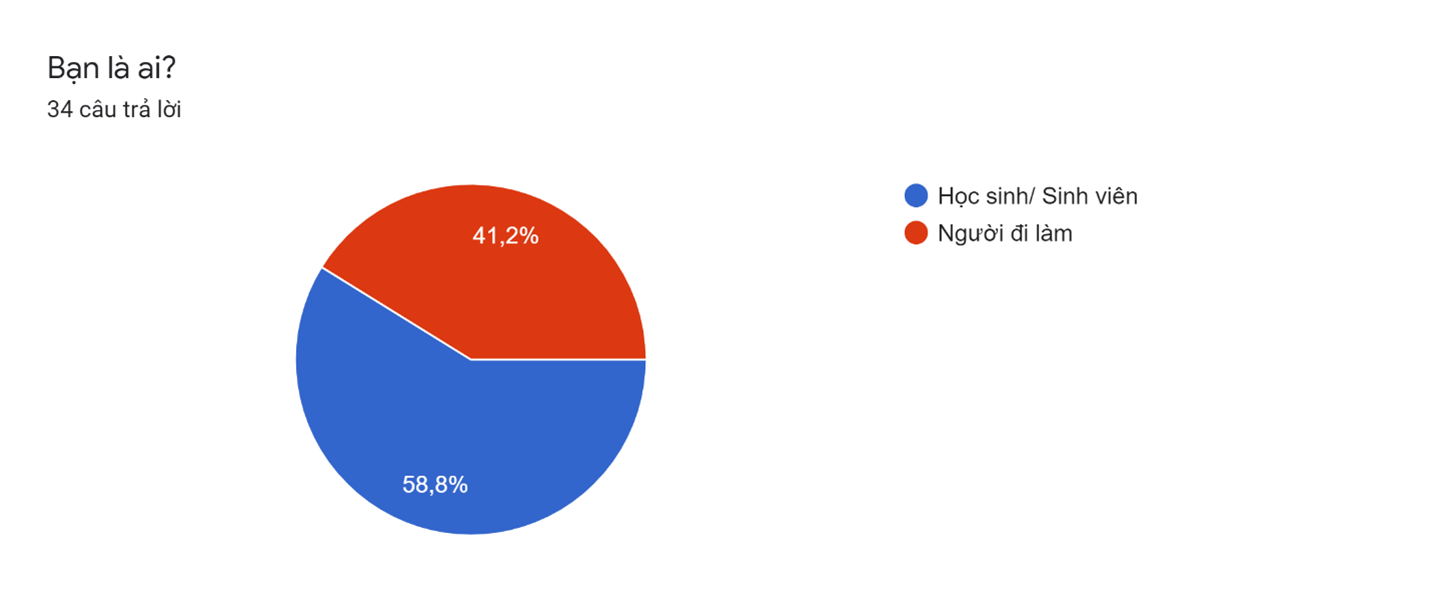
\includegraphics{images/survey1}
\caption{Thống kê đối tượng đang là sinh viên hoặc đã đi làm }
\label{fig:survey1}
\end{figure}
Phần lớn đối tượng tham gia khảo sát là sinh viên chiếm 58.8\% và đối với đối tượng là người đã đi làm thì chiếm 41.2%\\
\pagebreak
\subsection{Bạn hoạt động trong lĩnh vực nào?}
\begin{figure}[htp]
\centering
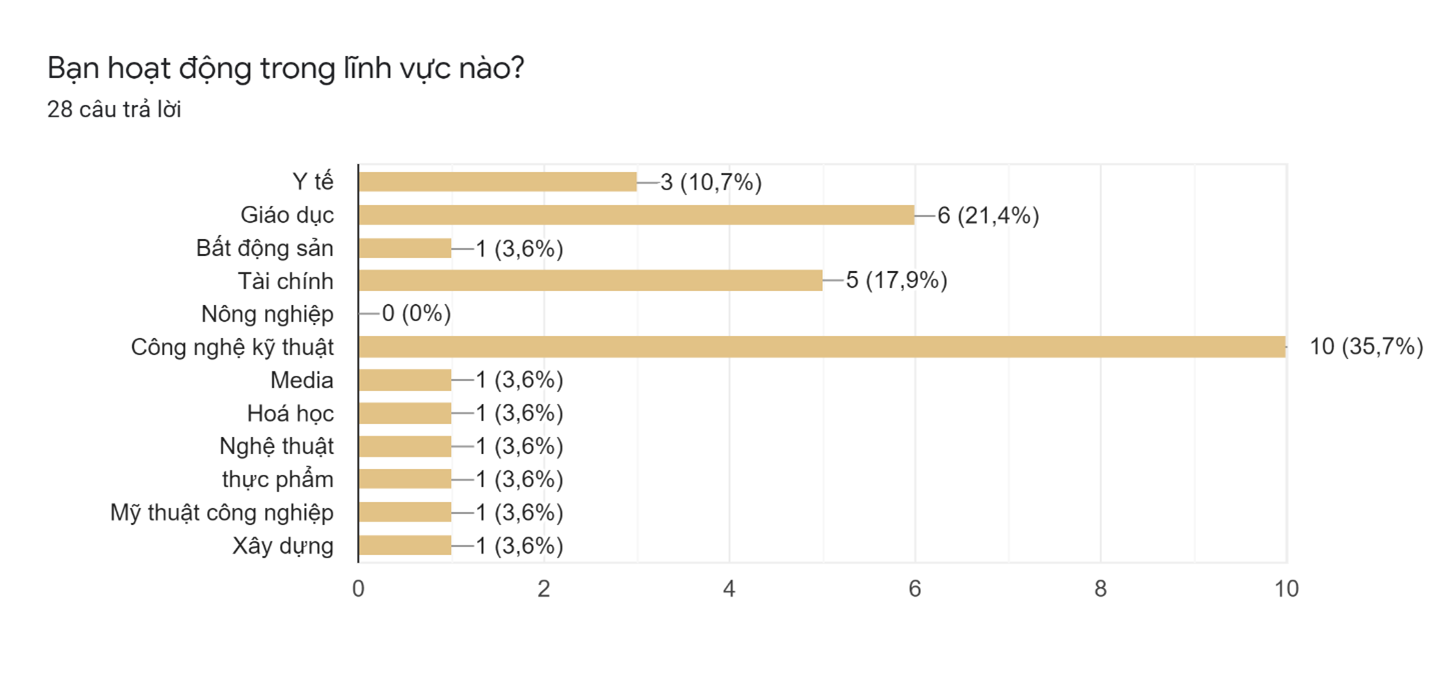
\includegraphics{images/survey2}
\caption{Thống kê đối tượng đang hoạt động trong lĩnh vực nào}
\label{fig:survey2}
\end{figure}

Qua khảo sát cho thấy, người tham gia khảo sát đang hiện hoạt động trong rất nhiều lĩnh vực như Y tế, Giáo dục, Công nghệ kỹ thuật, tài chính chiếm phần trăm khá cao trong tổng số lượng ngành có đưa ra để khảo sát.\\
\pagebreak
\subsection{Bạn đã từng gặp những vấn đề liên quan đến luật pháp?}
\begin{figure}[htp]
	\centering
	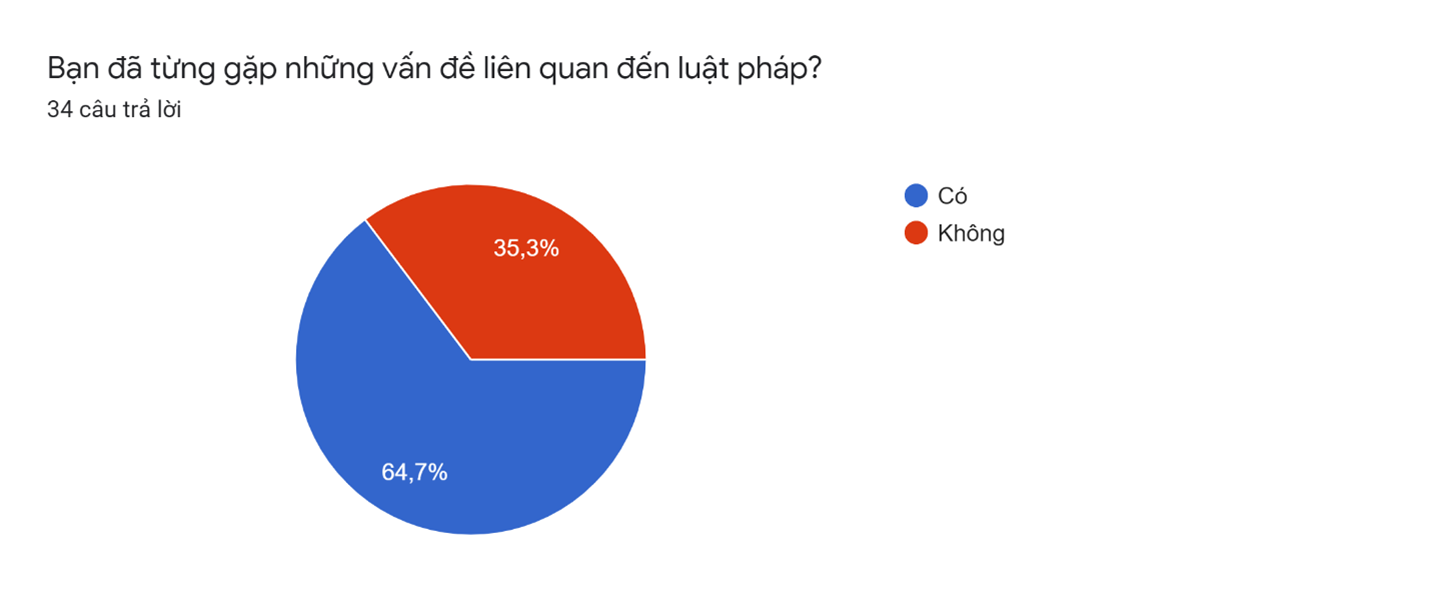
\includegraphics{images/survey3}
	\caption{Thống kê đối tượng có gặp những vấn đề liên quan đến pháp luật không?}
	\label{fig:survey3}
\end{figure}

Dựa vào kết quả khảo sát, có thể thấy đến gần 65\% số người được khảo sát gặp các vấn đề liên quan đến pháp luật, cho dù là học sinh, sinh viên hay người đi làm, học tập, làm việc trong các lĩnh vực khác nhau. Từ đây, có thể thấy nhu cầu tìm hiểu về pháp luật của người thực hiện khảo sát là rất lớn. \\
\pagebreak
\subsection{Bạn sử dụng phương thức nào để tra cứu pháp luật?}

\begin{figure}[htp]
	\centering
	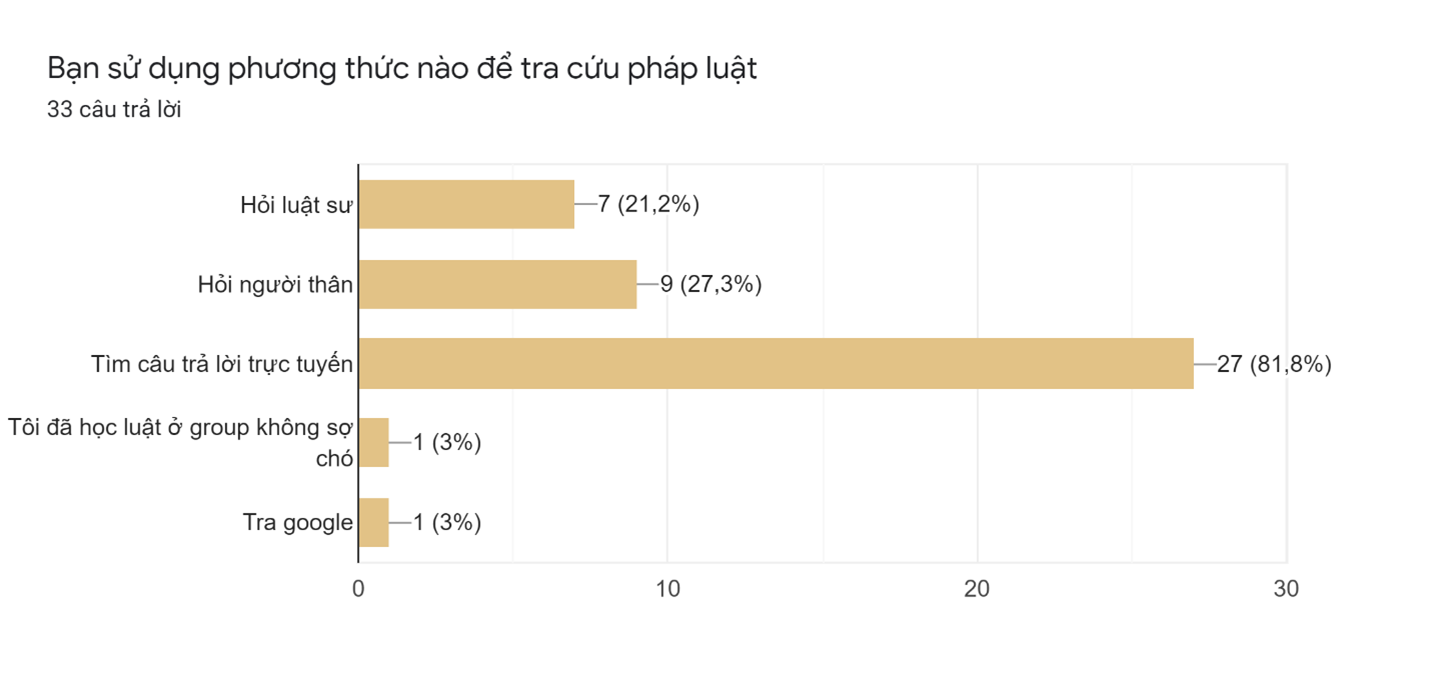
\includegraphics{images/survey4}
	\caption{Thống kê về phương thức nào của người dùng dùng để tra cứu pháp luật}
	\label{fig:survey4}
\end{figure}

Biểu đồ trên cho thấy các phương thức mà người khảo sát sử dụng để tìm hiểu về luật pháp. Đây là câu hỏi người thực hiện khảo sát có thể chọn nhiều phương án, trong đó, có thể thấy rằng người dùng có nhiều phương thức để tra cứu như hỏi luật sư, hỏi người thân,… nhưng đa số vẫn ưa thích tìm câu trả lời trực tuyến thông qua các trang web về pháp luật hoặc tìm trên Google.\\
\pagebreak
\subsection{Bạn thường tra cứu trên trang web pháp luật nào?}

\begin{figure}[htp]
	\centering
	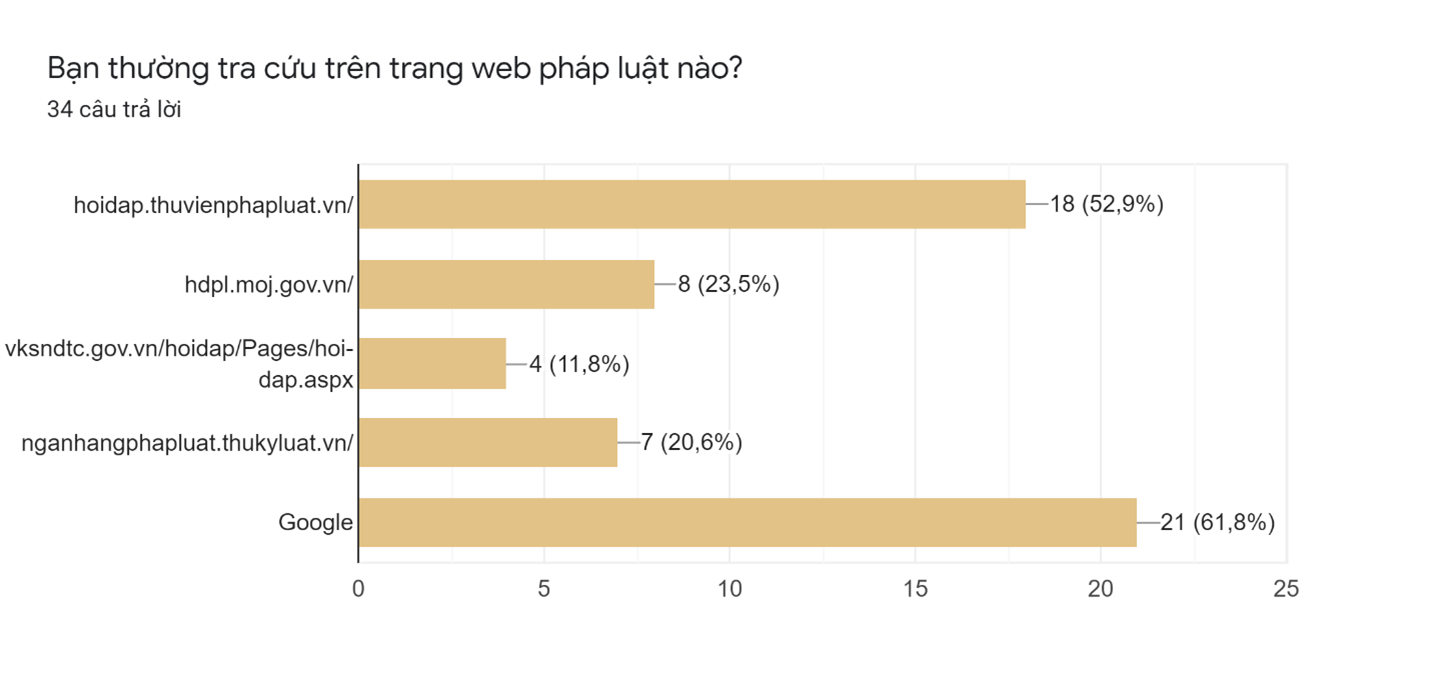
\includegraphics{images/survey5}
	\caption{Thống kê các trang web mà người dùng sử dụng để tra cứu thông tin luật pháp}
	\label{fig:survey5}
\end{figure}

Trên đây là những trang web chứa các thông tin về văn bản, câu hỏi về luật pháp. Người thực hiện khảo sát có thể sử dụng mỗi trang web khác nhau hoặc họ có thể kết hợp nhiều phương thức để tìm hiểu chi tiết, chính xác về vấn đề pháp luật họ gặp phải. Nhưng kết quả phần lớn vẫn là search thông tin của câu hỏi bằng Google.\\
\pagebreak
\subsection{Mức độ hài lòng khi sử dụng các trang web trên?}
\begin{figure}[htp]
	\centering
	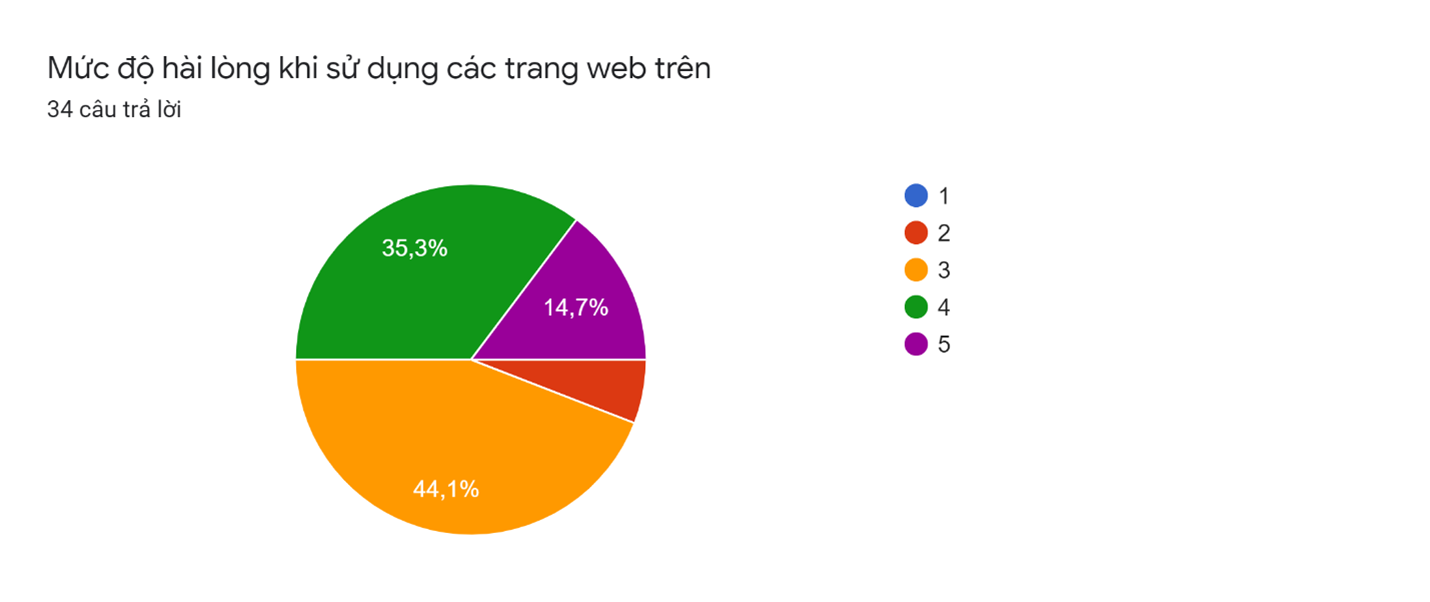
\includegraphics{images/survey6}
	\caption{Thống kê mức độ hài lòng khi sử dụng các trang web trên}
	\label{fig:survey6}
\end{figure}
Sau đó, người thực hiện khảo sát được yêu cầu cho cảm nhận về mức độ hài lòng khi họ sử dụng các trang web trên. Thang điểm từ 1 đến 5, tương ứng với các mức ‘rất tệ’, ‘tệ’, ‘vừa đủ’, ‘tốt’ và ‘rất tốt’. Từ biểu đồ trên, có thể thấy 44,1\% người dùng cảm thấy vừa đủ hài lòng khi sử dụng các trang web. 35,3\% cảm thấy tốt và 14,7\% cảm thấy rất tốt. Bên cạnh đó, họ còn đưa ra các nhận xét tích cực như ‘tiện lợi, nhanh chóng’ hay ‘khá chi tiết, đầy đủ’. Tuy nhiên, có một số nhận xét không hài lòng như khi sử dụng Google để tìm kiếm thông tin, kết quả trả về nhiều, tốn thời gian hoặc có người cho rằng các vấn đề về pháp luật của mỗi người khác nhau nhưng các trang web chỉ đưa ra những câu trả lời chung, khó có thể giải quyết mọi vấn đề.  \\

\subsection{Nhận xét của bạn khi sử dụng các trang web trên}
Mục này người khảo sát trả lời quá ít nên không thể thống kê.

\section{Bài Toán Liên Quan}
Qua quá trình tìm kiếm, tìm hiểu thì nhóm rút ra được để giải quyết được yêu cầu của hệ thống thì sẽ cần giải được các bài toán nhỏ liên quan như sau:
\begin{itemize}
	\item Thu thập giữ liệu về pháp luật từ các trang web chuyên về pháp luật
	\item Mã hoá dữ liệu câu hỏi - Xử lý ngôn ngữ tự nhiên
	\item So sánh tìm ra sự tương đồng giữa các câu
	\item Xây dựng model train trên dữ liệu Pháp luật     
\end{itemize}

\pagebreak
